\section{Design}
\label{sec:Design}

\subsection{Overview} 
This section discusses the design of the project including technologies used, classes, database schema, and user interface.

\subsection{Technologies}
This project uses a combination of ASP.NET Core MVC and Unity XR. The Course Creator was developed with the former and the Virtual Reality Orienteering was developed with the latter.

\subsubsection{Course Creator}
ASP.NET Core MVC \qquote{is a lightweight, open source, highly testable presentation framework optimized for use with ASP.NET Core.}{dotnetcoremvc} ASP.NET Core is the underlying framework that enables development. ASP.NET Core \qquote{is a cross-platform, high-performance, open-source framework for building modern, cloud-enabled, Internet-connected apps.}{dotnetcore}.\\
\\
The MVC in ASP.NET Core MVC stands for Model-View-Controller. MVC is an architectural pattern which separates an application into three main components: Models, Views, and Controllers. This separation helps achieve a ``separation of concerns", which asserts ``that software should be separated based on the kinds of work it performs" \cite{separationOfConcerns}. Models represent the data structure, independent of the user interface. Models are responsible for data, logic, and rules of the application. Views represent the user interface and information. Views are responsible for presenting content with minimal logic. Controllers represent the logic and actions for models and views. Controllers are responsible for responding to user input and preforming operations. In summary, models are what it is, views are for what it looks like, and controllers are for how it behaves. \\
\\
ASP.NET Core MVC was chosen because of the developer's prior experience and the extensive functionalities that the framework provides. ASP.NET Core MVC is open-source and multi-platform, supporting Windows, macOS, and Linux out of the box. \\
\\
ASP.NET Core MVC provides routing which is a useful URL-mapping component. Routing provides for easy link generation without regard to the actual file structure.\\
\\
ASP.NET Core MVC also provides model binding on requests. This makes incoming and outgoing requests easy to process or generate without further processing. Model validation is also built-in using data annotation attributes. These are pre-built or custom attributes within the model that validate on the fly rather than requiring explicit checking. This allows for guaranteeing the state of the model before further processing. \\
\\ 
Dependency injection is also supported, which is a key feature for building the controllers. Dependency Injection (DI) is a software design pattern, \qquote{which is a technique for achieving Inversion of Control (IoC) between classes and their dependencies.}{dependencyInjection} A dependency is an object that another object depends on. When a class depends on another class, future changes become problematic. Dependency Injection solves this by using an interface to abstract the dependency, registering the dependency in a service container, and then injects the dependency when needed.\\
\\
ASP.NET Core MVC provides filters which can be placed on controllers so that all actions must meet this filter. Oftentimes filters are added for exception handling or authorization. This way instead of each action requiring authorization, one can require the entire controller with all actions to be authorized. \\
\\
ASP.NET Core MVC is also a great platform for building Web APIs. HTTP content-negotiation with common data formats such as JSON or XML is already supported. \\
\\
The Razor view engine is another key advantage for ASP.NET Core MVC. Razor view engine is a compact and easy template markup language used for defining views with embedded \C code. Razor can be used to dynamically generate web content with a mix of server side and client side code. Tag Helpers are also used with Razor to facilitate creating and rendering HTML. Tag Helpers bind to certain HTML elements and vastly improves their use cases.\\
\\
Another tool used to aid in development was Bootstrap. Bootstrap is a CSS framework that helps standardize easily making changes to the look of websites and applications. Bootstrap makes use of a grid system comprised of 12 grid boxes evenly split across a page. These grids can be coalesced to form sections within the web page. Bootstrap has built-in functionality that makes web pages mobile friendly.\\
\\
ASP.NET Core MVC also provides a database object-relational mapper (O/RM) tool called Entity Framework Core. Entity Framework Core provides a ``code first" experience to create database entity models by writing code. This cuts down on the boilerplate code required for making database connections. The database can be accessed and queried using LINQ, Language-Integrated Query, a set of technologies based on the integration of query capabilities directly into the \C language. Entity Framework Core makes committing changes to the database simple with automatic change tracking.

\subsubsection{Virtual Reality Orienteering}
Unity is a cross-platform game engine developed by Unity Technologies with the goal to provide developers with the tools to make game development simple. Unity supports a vast variety of platforms and user experiences. These tools extend to desktop, mobile, console, and virtual reality with support for 2D, 3D, and other experiences. It's also used in other areas outside of game development such as film, engineering, architecture, and automotive modeling. This makes Unity a popular choice, not only for the developer of this project, but for the world at large. \qquote{In the fourth quarter of 2021, Unity had, on average, 3.9 billion monthly active end users who consumed content created or operated with its solutions.}{unityNumbers} \\
\\
The basic components of a game developed in Unity are GameObjects, Assets, Scenes, and Scripts. Every object in a game is a GameObject.\\
\\
Assets are reusable items that can be used throughout the game. They can be of any file type that Unity supports, such as a 3D model, audio file, image. Oftentimes these assets come from outside Unity, created by the developer or other developers which are found in the Asset Store. \\
\\
Scenes contain the objects of the game. Oftentimes these are split into logical groupings such as main menu, individual levels, or the environment. \\
\\
Scripts are what controls the behavior of the GameObjects. Without scripts the game would be static and have no interaction or logic. Unity supports \C natively and is the standard used for scripting. A new script has two functions, \lstinline{Start()} and \lstinline{Update()}. \lstinline{Start()} is called once by Unity before gameplay begins which is used to setup initial configurations. \lstinline{Update()} is called once per frame update for the GameObject. This is used to handle anything that needs to be done over time in the gameplay, such as movement, triggering actions, or responding to user input.  \\
\\
\begin{lstlisting}[caption=New Script in Unity]
using UnityEngine;
using System.Collections;

public class NewBehaviourScript : MonoBehaviour {

	// Use this for initialization
	void Start()
	{
	
	}
	
	// Update is called once per frame
	void Update() 
	{
	
	}
}
\end{lstlisting}

Unity XR Interaction Toolkit is a cross-platform plugin used for virtual, mixed, and augmented reality. XR Interaction Toolkit provides easy built-in functionality to select, grab, throw, rotate objects within a VR scene. This also extends to the UI interactions and the haptic feedback that comes with it. The ability to look around and move within the worldspace is also provided with this plugin. As this project uses a HTC Vive headset, OpenXR was the targeted development platform. OpenXR is an open standard that targets a wide array of virtual reality devices.

\subsection{Class Diagrams}

\subsubsection{Course Creator}

Figure \ref{Course Creator UML Class Diagram} shows the class diagram. Each component of the Course Creator is comprised of a model, DbContext, and controller. The model describes what each object represents with minimal processing. The DbContext is the connection to the database. Entity Framework Core uses these DbContext classes linked with the models to provide the database operations. The controller provides the implementation and logic needed to handle operations. The controller makes use of the DbContexts to make changes to the data. The DbContext and Controller classes use Dependency Injection to separate the data and processing layers without needing to know the implementation details of each. The Startup class not shown links up the Dependency Injection needed for the DbContext and Controller. 

\begin{figure}[htb]
	\centering
	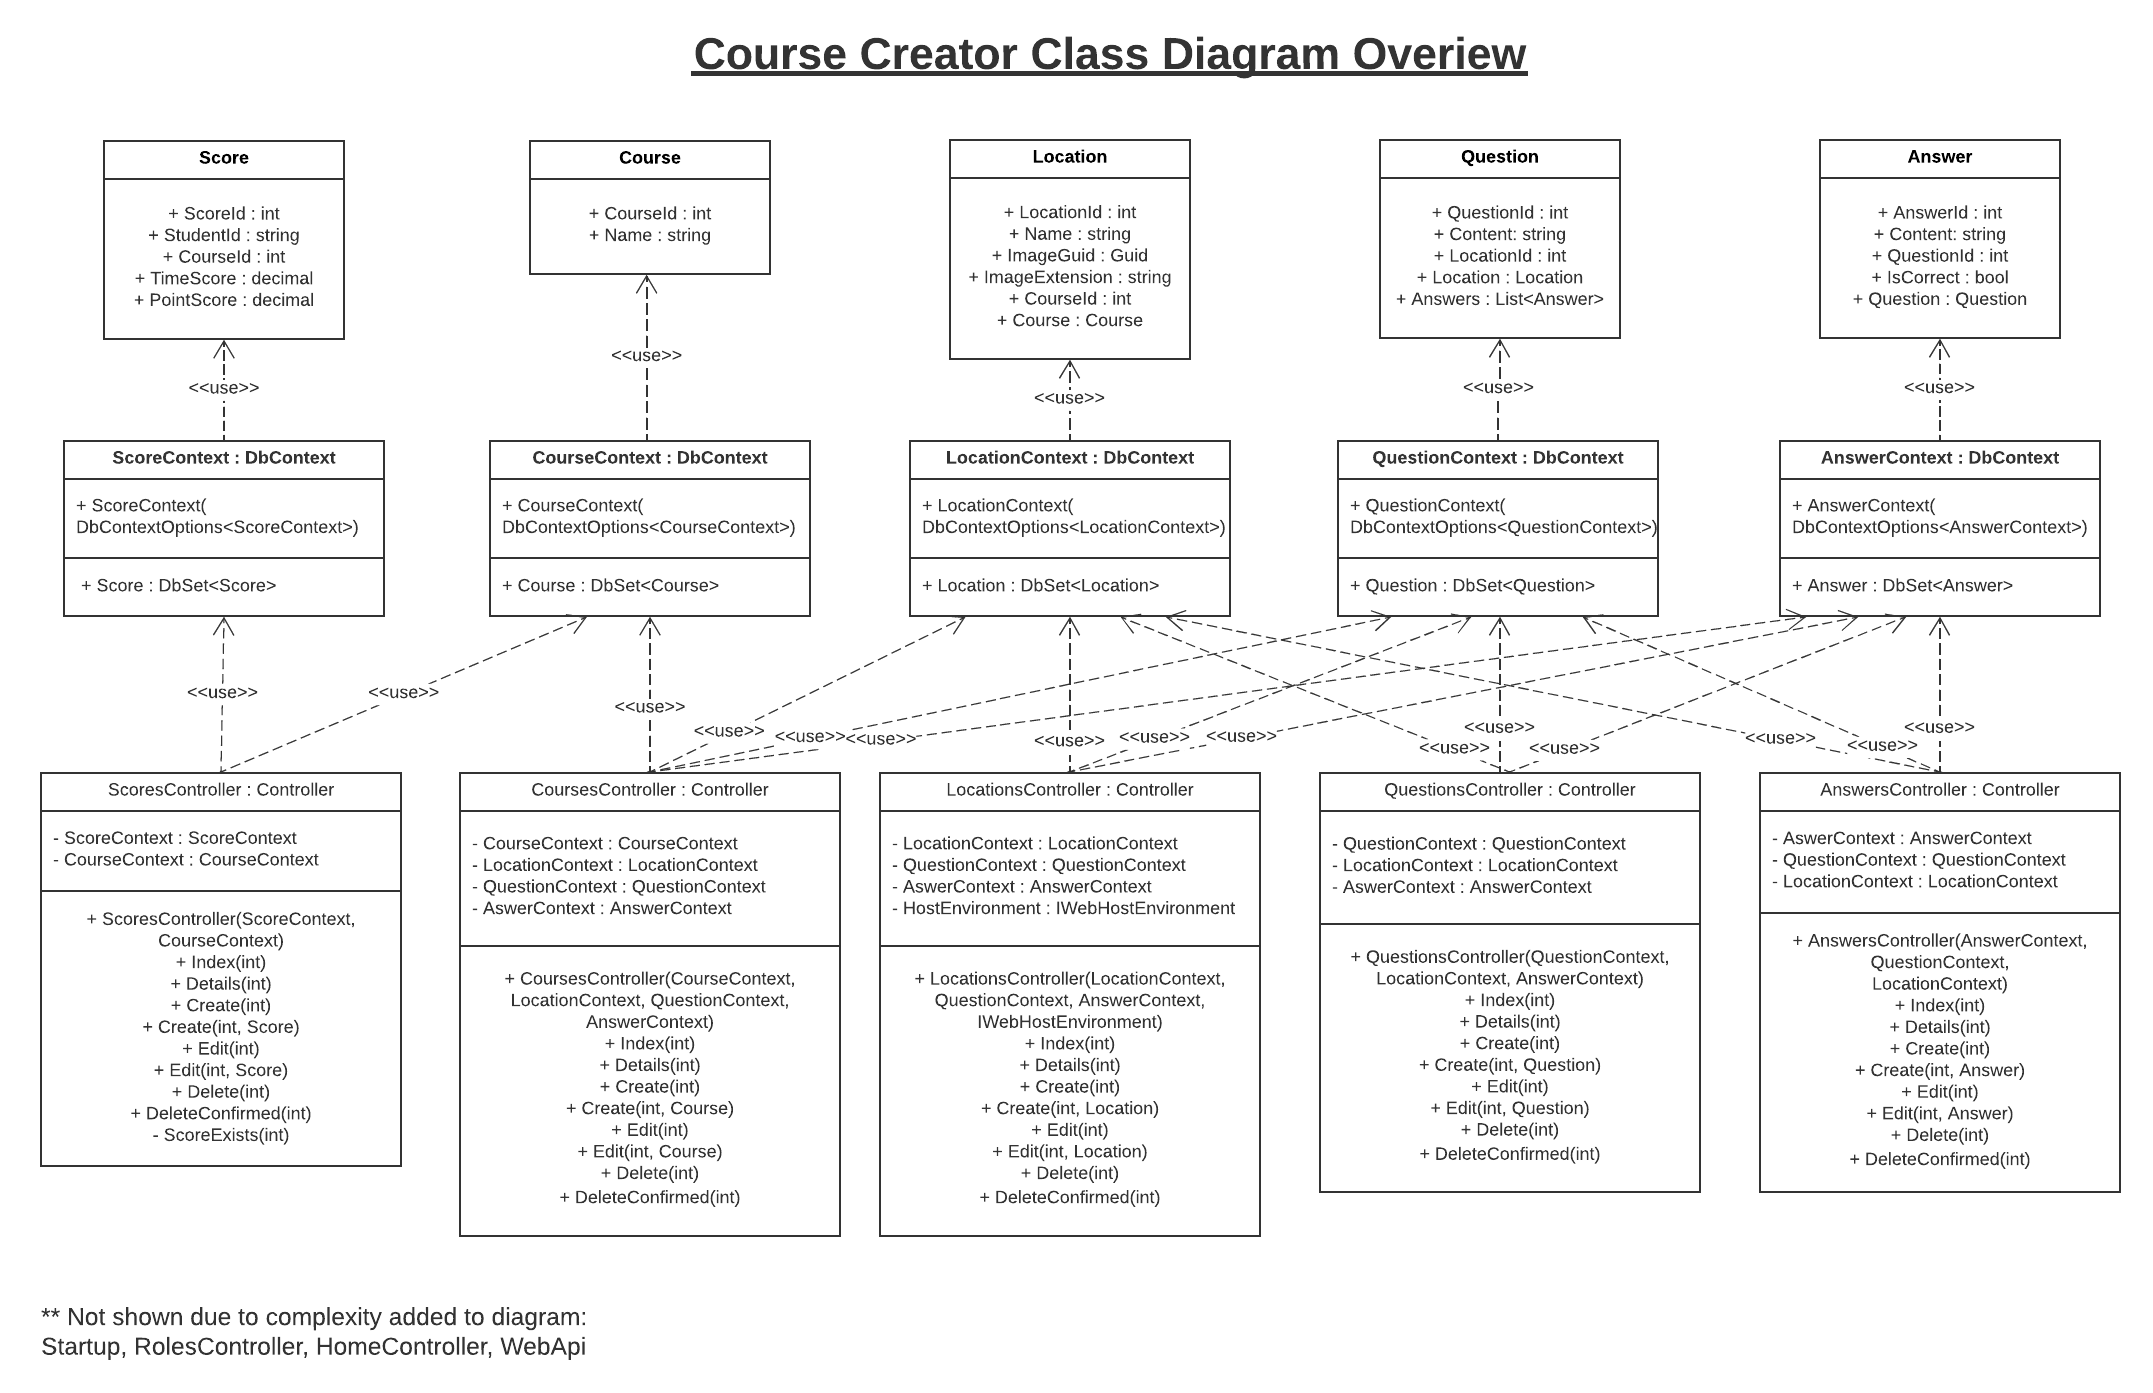
\includegraphics[width=.9\textwidth]{Design/assets/course-creator-class-diagram.png}
	\caption[Course Creator UML Class Diagram]{\label{Course Creator UML Class Diagram}Course Creator UML Class Diagram}
\end{figure}
\clearpage

\subsubsection{Virtual Reality Orienteering}

Figure \ref{Virtual Reality Orienteering UML Class Diagram} shows the class diagram. The VRInputModule contains much of the logic and operations needed for the Virtual Reality Orienteering program. The VRInputModule also meditates the Pointer and ButtonTransitoner classes so that buttons respond to a click action. The VRInputModule calls the EnvironmentLibrary for loading new locations. The EnvironmentLibrary makes calls to the Web API and transforms the returned data into usable formats for the VRInputModule and uses the SkyBoxController to display the 360 Photos in the worldspace. 

\begin{figure}[htb]
	\centering
	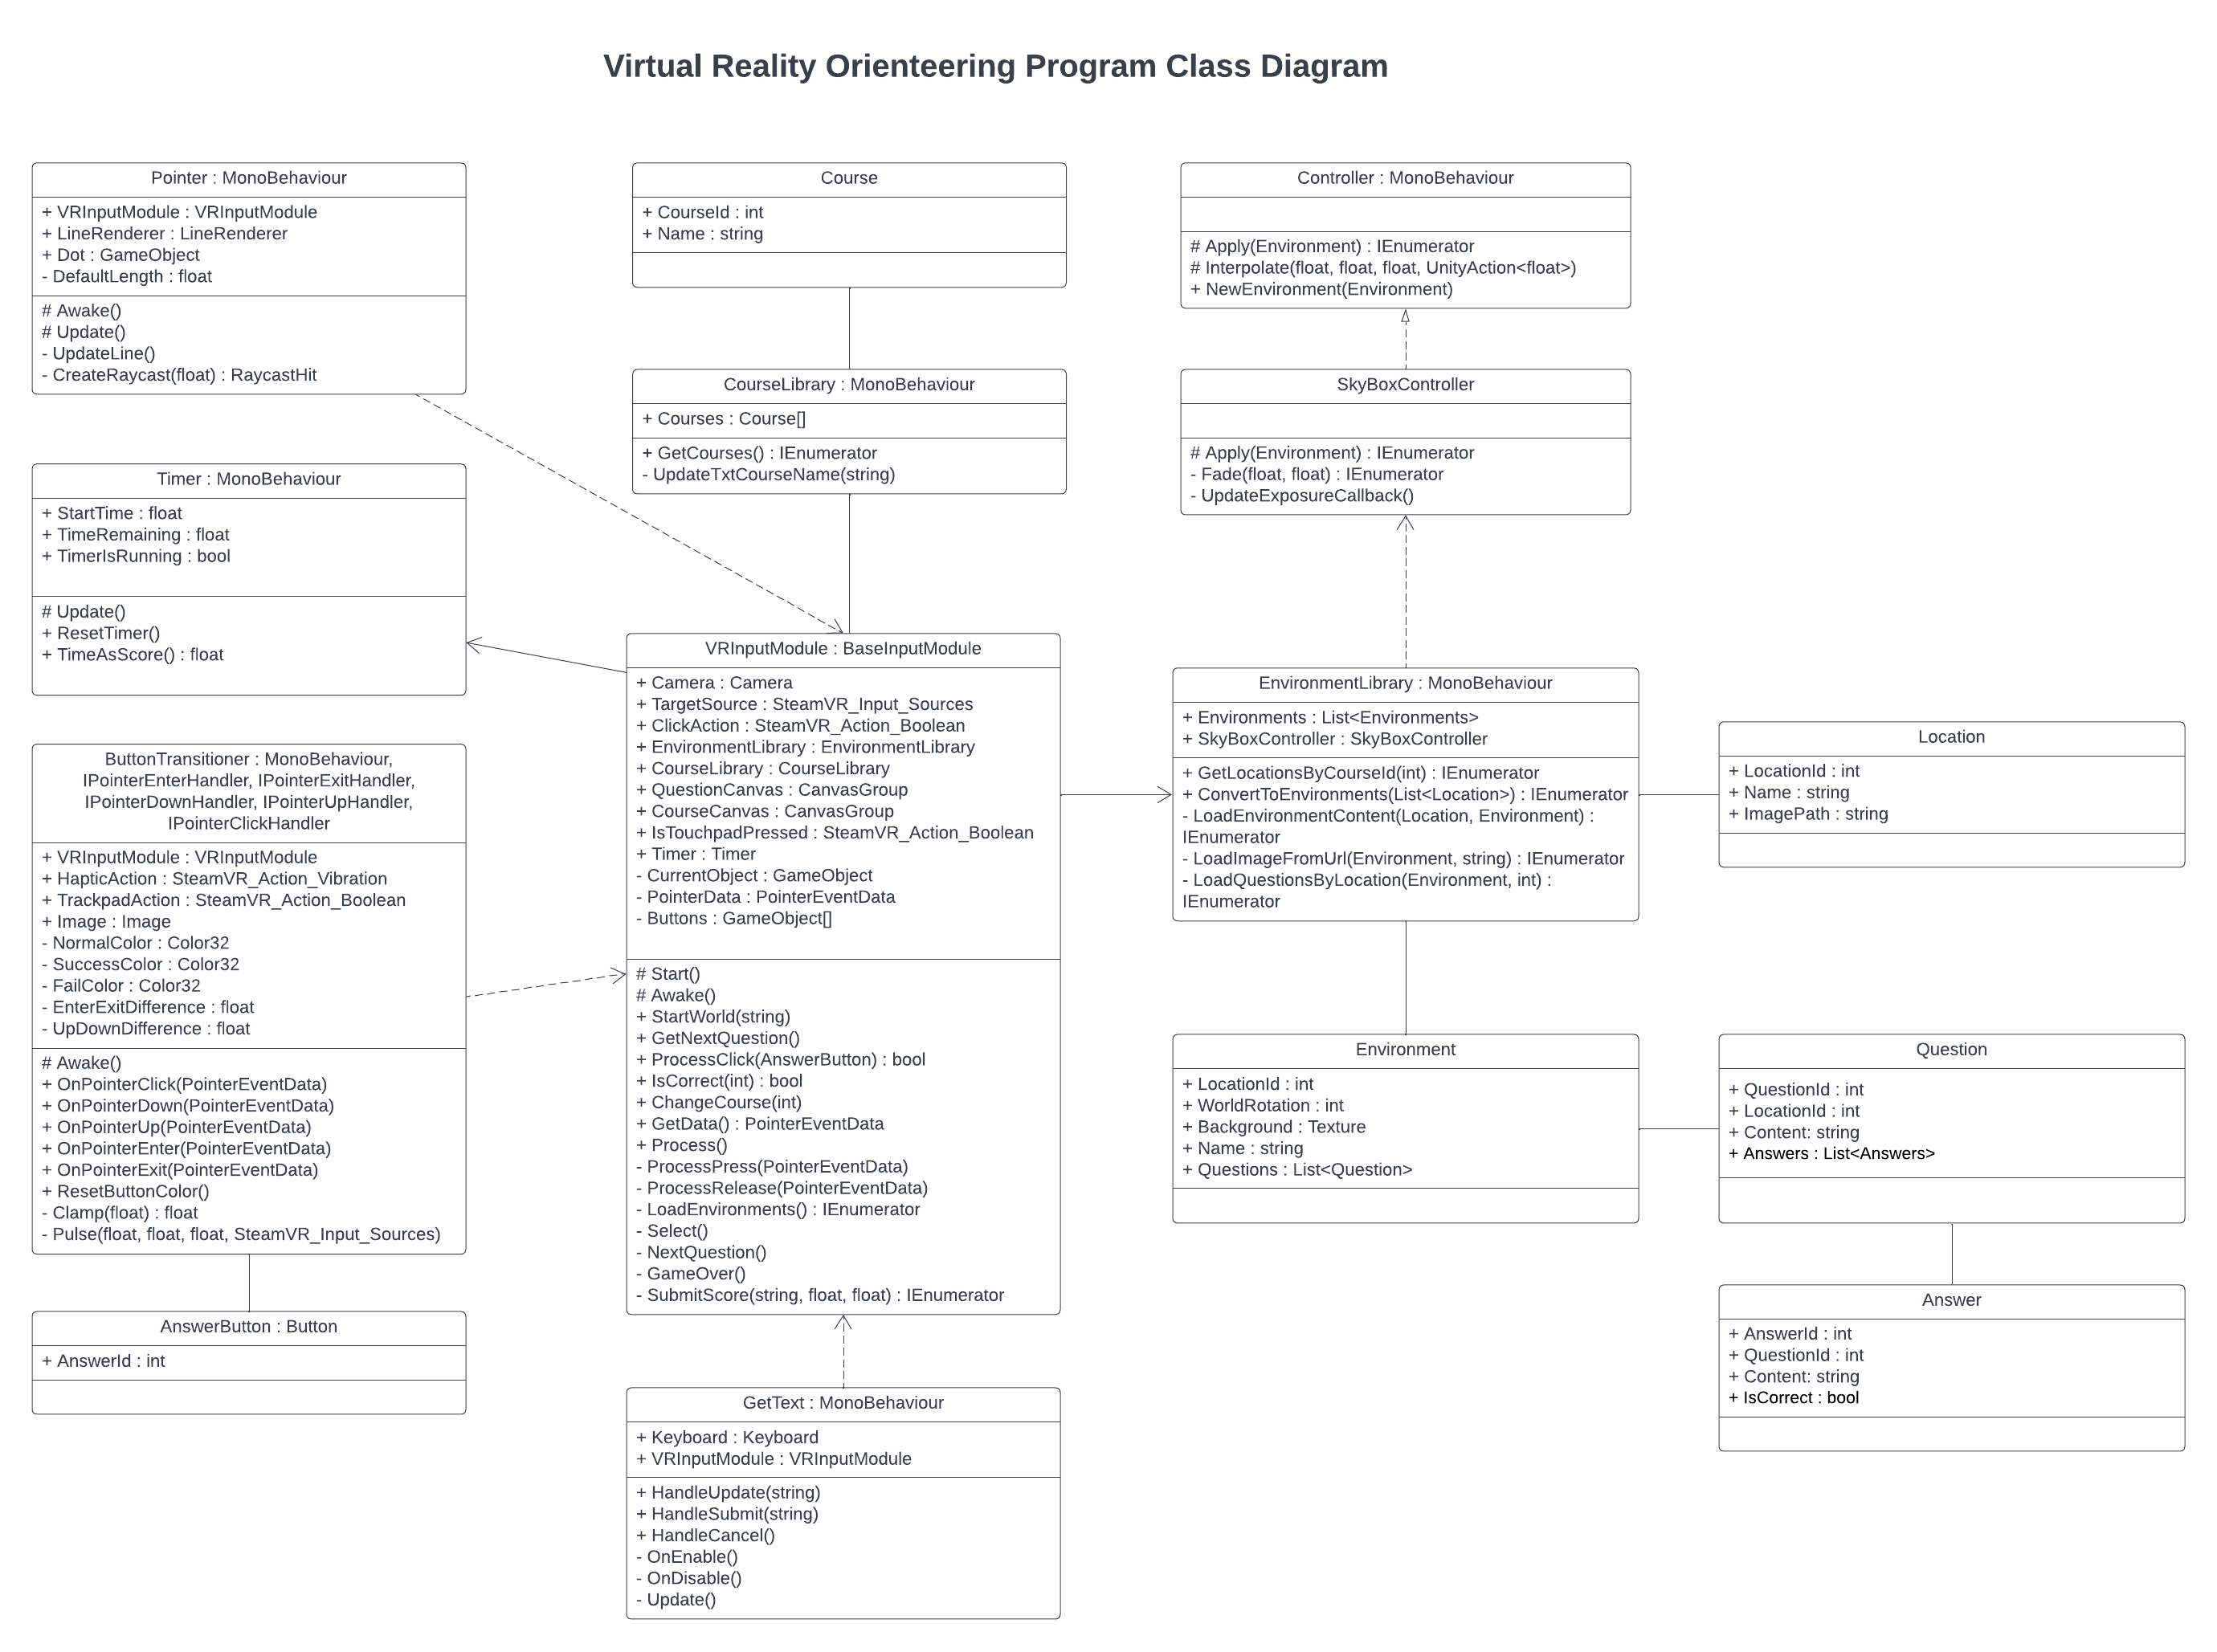
\includegraphics[width=.9\textwidth]{Design/assets/vr-class-diagram.png}
	\caption[Virutal Reality Orienteering UML Class Diagram]{\label{Virtual Reality Orienteering UML Class Diagram}Virtual Reality Orienteering UML Class Diagram}
\end{figure}

\subsection{Database}
The database uses Microsoft's SQL Server. SQL Server is the de facto used for .NET projects.  SQL Server is a relation database management system which manages and stores information. The standard tool for working with SQL Server is SQL Server Management Studio which makes database changes and transactions easy. Transparent Data Encryption (TDE) encrypts data files at rest. This means that any data files stored are encrypted preventing any malicious attempts to read the database.
\clearpage
\subsubsection{Database Schema}
Figure \ref{ER Diagram} shows the ER Diagram for the database that the project uses. Each component of a course has a one-to-many relationship with each parent object. This means that a course has many locations, a location has many questions, a question has many answers.
\begin{figure}[htb]
	\centering
	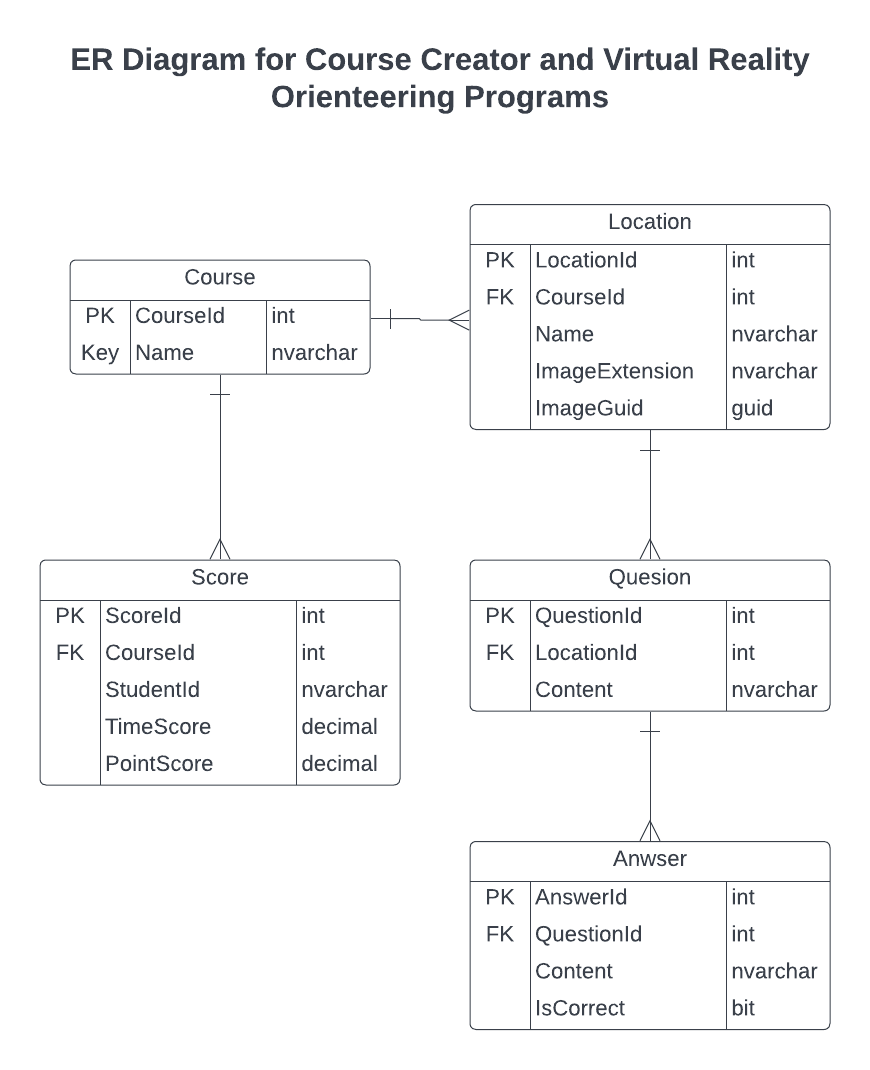
\includegraphics[width=.6\textwidth]{Design/assets/capstone-er-diagram.png}
	\caption[ER Diagram]{\label{ER Diagram}ER Diagram}
\end{figure}
\subsection{Communication between Programs}
This project comprises of two separate programs which must communicate with each other, and do so securely. The Course Creator has a RESTful Web API which requires Basic Authentication to make calls to.  Basic Authentication requires a username and password over an HTTP connection. Using just an HTTP connection is not secure though, as the username and password are sent over in plaintext. This means any malicious user can sniff the network and easily obtain the credentials. To counter this the project requires a secure connection using HTTPS, with the `S' meaning secure. An HTTPS connection encrypts any data sent over it; thereby securing the Basic Authentication credentials. \\
\\
The RESTful Web API provides predefined endpoints for authorized users to use with REST calls. REST stands for REpresentational State Transfer and is a architectural standard for communication on the web. REST is stateless, meaning that the server does not need to know about what state the client is or vice versa. This allows for communication without needing to know the previous messages. A REST request usually is comprised of an HTTP verb, header, URI path, and an optional body containing data. The four basic HTTP verbs are GET, POST, PUT, and DELETE. GET retrieves data or a specific resource. POST creates new data or a new resource. PUT updates data or a specific resource. Finally, DELETE removes data or a specific resource. The header is used for carrying pertinent information about the request being made. This includes the authorization, cookies, caching, and other logistical information for fulfilling the request. The REST requests consume or return data in JSON which is a standard data-interchange format. JSON is easy for humans to read and simple for computers to parse and generate.


